
\chapter{图片, 表格, 枚举}

%%%%%%%%%%%%%%%%%%%%%%%%%%%%%%%%%%%%%%%%%%%%%%%%%%%%%%%%%%%
%%%%%%%%%%%%%%%%%%%%%%%%%%%%%%%%%%%%%%%%%%%%%%%%%%%%%%%%%%%

\section{图片}

这里是overleaf的插入图片的学习文档。

\href{https://www.overleaf.com/learn/latex/Inserting_Images}{插入图片}

\href{https://www.overleaf.com/learn/latex/Positioning_images_and_tables}{图片和表格的位置}

几乎所有的文档都需要图片. 要插入图片需要\imp{graphicx}包。

\begin{figure}[!h]
	\centering
	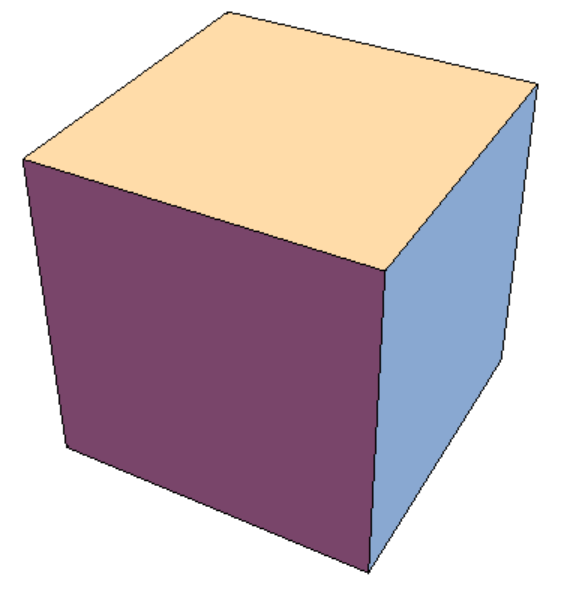
\includegraphics[width=0.3\textwidth]{figures/cube.png}
	\caption{A figure caption beneath the figure for description of the depicted concept which sometimes can be very long}
	\label{fig:ft_fig_firstfig}
\end{figure}

在 \autoref{fig:ft_fig_firstfig}中, 绘制了一个PNG图片。 

同样, 如果使用dvips和ps2pdf来编译,也可插入EPS 图片
使用\imp{listoffigures},打印所有图片目录。

\begin{figure}[!h]
    \centering
    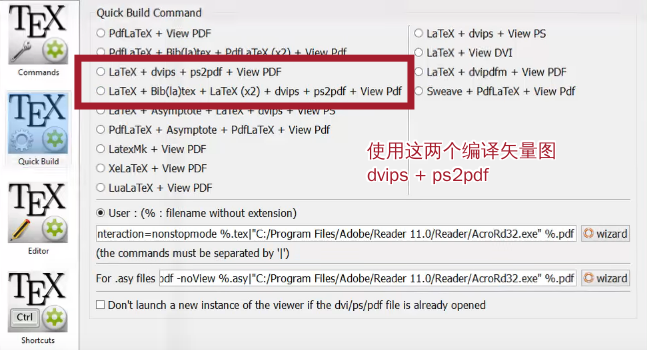
\includegraphics[width=0.8\linewidth]{figures/vector_figure.png}
    \caption{矢量图的编译方式}%
    \label{fig:vector_figure}
\end{figure}
%%%%%%%%%%%%%%%%%%%%%%%%%%%%%%%%%%%%%%%%%%%%%%%%%%%%%%%%%%%
%%%%%%%%%%%%%%%%%%%%%%%%%%%%%%%%%%%%%%%%%%%%%%%%%%%%%%%%%%%

\section{表格}

这里有一个很好的{LaTeX}表格生成网址,\href{https://www.tablesgenerator.com/}{LaTeX 表格生成网址}

下面就是一个表格\autoref{ft_tab_ex}.

\begin{table}[!h]
	\centering
	\begin{tabular}{l|c|l}
	\hline \hline
	
		& Property 1
		& Property 2\\ \hline
	Criterion 1
		& 764
		& 23546 \\
	Criterion 2
		& 3
		& 34 \\
	\hline \hline
	\end{tabular}
	\caption{Exemplary table}
	\label{ft_tab_ex}
\end{table}

有些时候需要非常长的表格,长度都超过一页。如果是这种情况,使用包\imp{longtable},例如下面这种情况:


\begin{center}
\begin{longtable}{l|l|l}

% \baselinestretch{1.5}

 \hline \hline
 $i^3$ & $2i^3$ & $3i^3$ \bigstrut \\ \hline
 \endfirsthead
 
 \multicolumn{3}{c}{\tablename\ \thetable{} -- information message on top} \\
 \hline
 $i^3$ & $2i^3$ & $3i^3$ \bigstrut \\ \hline 
 \endhead
 
 \hline
 \multicolumn{3}{c}{Foot information} \\ \hline
 \endfoot
 
 \hline \hline
 \caption{Long Table}
 \label{lt}
 \endlastfoot
 
 1 & 2 & 3 \\
 8 & 16 & 24 \\
 27 & 54 & 81 \\
 64 & 128 & 192 \\
 125 & 250 & 375 \\
 216 & 432 & 648 \\
 343 & 686 & 1029 \\
 512 & 1024 & 1536 \\
 729 & 1458 & 2187 \\
 1000 & 2000 & 3000 \\
 1331 & 2662 & 3993 \\
 1728 & 3456 & 5184 \\
 2197 & 4394 & 6591 \\
 2744 & 5488 & 8232 \\
 3375 & 6750 & 10125 \\
 4096 & 8192 & 12288 \\
 4913 & 9826 & 14739 \\
 5832 & 11664 & 17496 \\
 6859 & 13718 & 20577 \\
 8000 & 16000 & 24000 \\
 9261 & 18522 & 27783 \\
 10648 & 21296 & 31944 \\
 12167 & 24334 & 36501 \\
 13824 & 27648 & 41472 \\
 15625 & 31250 & 46875 \\
 17576 & 35152 & 52728 \\
 19683 & 39366 & 59049 \\
 21952 & 43904 & 65856 \\
 24389 & 48778 & 73167 \\
 27000 & 54000 & 81000 \\
 29791 & 59582 & 89373 \\
 32768 & 65536 & 98304 \\
 35937 & 71874 & 107811 \\
 39304 & 78608 & 117912 \\
 42875 & 85750 & 128625 \\
 46656 & 93312 & 139968 \\
 50653 & 101306 & 151959 \\
 54872 & 109744 & 164616 \\
 59319 & 118638 & 177957 \\
 64000 & 128000 & 192000 \\
 68921 & 137842 & 206763 \\
 74088 & 148176 & 222264 \\
 79507 & 159014 & 238521 \\
 85184 & 170368 & 255552 \\
 91125 & 182250 & 273375 \\
 97336 & 194672 & 292008 \\
 103823 & 207646 & 311469 \\
 110592 & 221184 & 331776 \\
 117649 & 235298 & 352947 \\
 125000 & 250000 & 375000 \\
\end{longtable}
\end{center}

所有的表格可以用\imp{listoftables}来打印。

%%%%%%%%%%%%%%%%%%%%%%%%%%%%%%%%%%%%%%%%%%%%%%%%%%%%%%%%%%%
%%%%%%%%%%%%%%%%%%%%%%%%%%%%%%%%%%%%%%%%%%%%%%%%%%%%%%%%%%%

\section{枚举}

使用数字的枚举可以用\imp{enumerate} 环境:
\begin{enumerate}
\item
	Some important stuff
\item
	More stuff
\end{enumerate}
在使用\imp{enumerate} 包以后, 可以使用一些选项,e.g.,
\begin{enumerate}[a)]
\item
	Some important stuff
\item
	More stuff
\end{enumerate}
or 
\begin{enumerate}[~~~1)]
\item
	Some important stuff
\item
	More stuff
\end{enumerate}

没有数字关系的枚举可以用 \imp{itemize}环境。
\begin{itemize}
\item
	Some important stuff
\item
	More stuff
\end{itemize}

关于 \imp{itemize}里序号的形式 (上面的例子): latex默认生成的简单列表, 
默认为一个小圆点, 而我们在写文章时可能想要一些不一样的列表符号, 
比如 -, * 之类的. 我们可以这样写:
\begin{itemize}
    \item[-] 吃饭
    \item[*] 睡觉
    \item[-] 躺下
\end{itemize}

%%%%%%%%%%%%%%%%%%%%%%%%%%%%%%%%%%%%%%%%%%%%%%%%%%%%%%%%%%%
%%%%%%%%%%%%%%%%%%%%%%%%%%%%%%%%%%%%%%%%%%%%%%%%%%%%%%%%%%%
%%%%%%%%%%%%%%%%%%%%%%%%%%%%%%%%%%%%%%%%%%%%%%%%%%%%%%%%%%%
